% {{{
\documentclass[a4paper, dvipdfmx, mathserif]{beamer}
% 印刷時には[]内に”handout”を追記する。
\usepackage{moreverb}
\usepackage{graphicx}
\usepackage{float}
\usepackage{wrapfig}
\usepackage{txfonts}
\usepackage{amsmath}
\usepackage{amssymb}
\usepackage{amsthm}
\usepackage{ascmac}
\usepackage{caption}
\usepackage{otf}

\bibliographystyle{junsrt}

\usetheme{Antibes}
% Hannover, boxes, default
\usecolortheme{seagull}
\usefonttheme{default} %{professionalfonts}
\useinnertheme{rectangles} % rounded rectangles
%%%%%%%%%%%%%%%% フレーム外側のテーマの選択(省略可)
%%\useoutertheme{default}
\useoutertheme{infolines}
%% \useoutertheme{miniframes}
%% \useoutertheme{smoothbars}
% \useoutertheme{sidebar}
%% \useoutertheme{split}
%% \useoutertheme{shadow}
%% \useoutertheme{tree}
%% \useoutertheme{smoothtree}
\setbeamertemplate{navigation symbols}{}
\setbeamertemplate{footline}[frame number]
\setbeamertemplate{frametitle}[default][center]
\setbeamertemplate{caption}[numbered]

\setbeamerfont{title}{size=\huge,series=\bfseries}
\setbeamerfont{subtitle}{size=\small,series=\bfseries}
\setbeamerfont{frametitle}{size=\large,series=\bfseries}

% \setbeamerfont{title}{size=\large}
% \setbeamerfont{frametitle}{size=\large}

% PDFのしおりが文字化けしないようにする
\usepackage{atbegshi}
\ifnum 42146=\euc"A4A2 \AtBeginShipoutFirst{\special{pdf:tounicode EUC-UCS2}}\else
\AtBeginShipoutFirst{\special{pdf:tounicode 90ms-RKSJ-UCS2}}\fi

\usepackage{hyperref}

\renewcommand{\familydefault}{\sfdefault}
\renewcommand{\kanjifamilydefault}{\gtdefault}
\renewcommand{\figurename}{図}
\renewcommand{\tablename}{表}

\newenvironment<>{varblock}[2][\textwidth]{%
\setlength{\textwidth}{#1}
\begin{actionenv}#3%
\def\insertblocktitle{#2}%
\par%
\usebeamertemplate{block begin}}
{\par%
\usebeamertemplate{block end}%
\end{actionenv}}

% "\vector{a}" でベクトル
\def\vector#1{\mbox{\boldmath \(#1\)}}

\hypersetup{breaklinks=true,
            bookmarks=true,
            pdfauthor={山﨑研M2 藤本將太郎},
            pdftitle={中間発表 -- 成長するひも状オブジェクトの折りたたみ機構について},
            colorlinks=true,
            citecolor=blue,
            urlcolor=black,
            linkcolor=black,
            pdfborder={0 0 0}}
\urlstyle{same}  % don't use monospace font for urls
% }}}
\title[中間発表]{成長するひも状オブジェクトの\\折りたたみについて}
\author[藤本]{山崎研M2 藤本將太郎}
\date{2016/07/08}

\begin{document}

\begin{frame}[plain]
    \vspace{2cm}
    \titlepage
    \vspace{1cm}
    {\tiny Online: \href{https://github.com/ssh0/growing-string/blob/master/doc/160708.pdf}{https://github.com/ssh0/growing-string/blob/master/doc/160708.pdf}}
  \end{frame}

\section{アウトライン} %{{{
\begin{frame}{アウトライン}

\begin{itemize}
\itemsep1pt\parskip0pt\parsep0pt
\item
  研究背景
\item
  研究目的
\item
  モデルの提案 + シミュレーション結果
  \begin{itemize}
    \itemsep1pt\parskip0pt\parsep0pt
    \item
      ひも状細胞を弾性体としてとらえるモデル

      \begin{itemize}
        \itemsep1pt\parskip0pt\parsep0pt
        \item
          自然長増大による成長
        \item
          自然長,バネ定数を一定に保つモデル
      \end{itemize}
    \item
      三角格子上で動くひも状オブジェクトのモデル
  \end{itemize}
\item
  今後の課題
\end{itemize}

\end{frame}
%}}}
\section{研究背景} %{{{
\begin{frame}{研究背景} %{{{

\emph{Bacillus subtilis}の栄養寒天培地上での成長パターンの研究

\begin{itemize}
\itemsep1pt\parskip0pt\parsep0pt
\item
  寒天の硬さと栄養濃度によって生成されるパターンの分類とモデル化

  \begin{itemize}
  \itemsep1pt\parskip0pt\parsep0pt
  \item
    1) \href{http://www.sciencedirect.com/science/article/pii/S0022519397904628}{K.
    Kawasaki, A. Mochizuki, M. Matsushita, T. Umeda, and N. Shigesada.
    Modeling spatio-temporal patterns generated bybacillus subtilis.
  Journal of Theoretical Biology, Vol. 188, No. 2, pp.~177-185, 1997.}
  \end{itemize}
\end{itemize}

\begin{figure}[htbp]
\centering
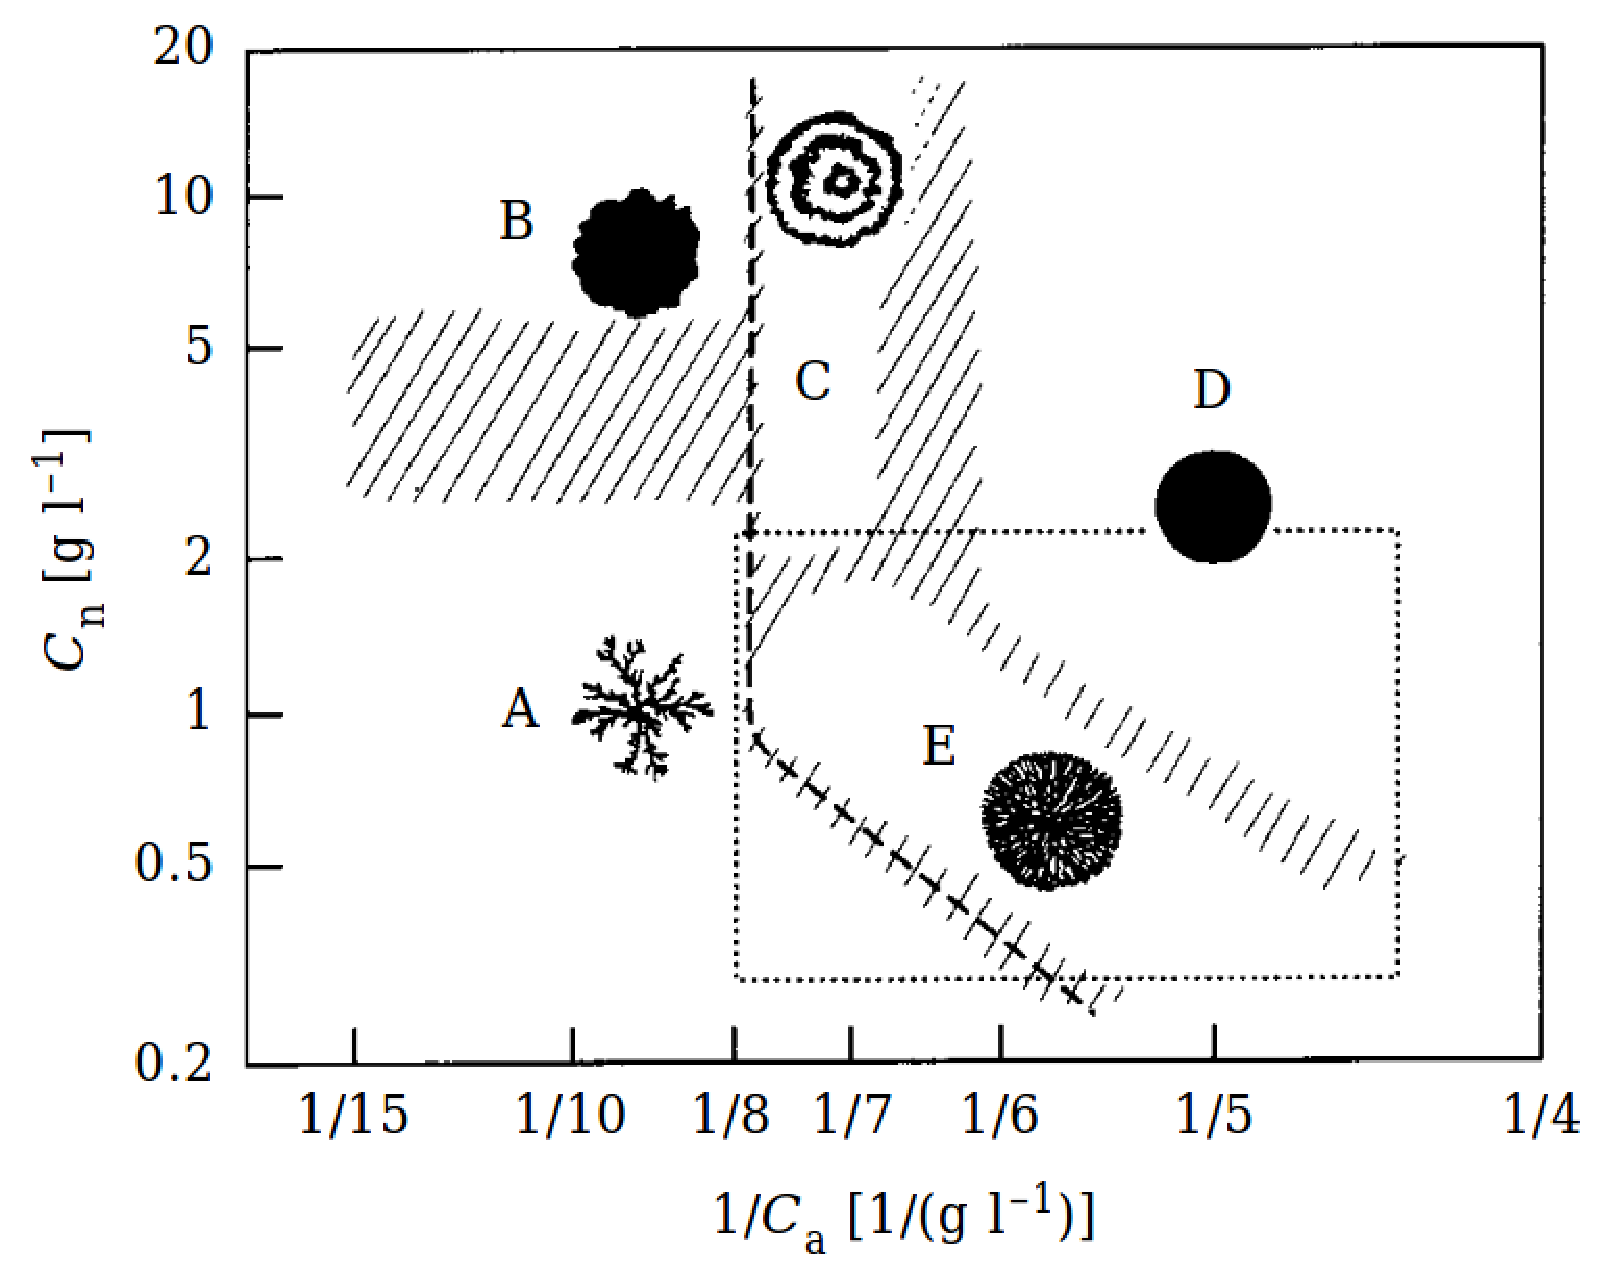
\includegraphics[width=0.4\textwidth]{../img/diagram.pdf}
\caption{寒天の硬さと栄養濃度によって生成されるパターン $^{1)}$}
\end{figure}

\end{frame}%}}}

\begin{frame}{研究背景} %{{{

\begin{itemize}
\itemsep1pt\parskip0pt\parsep0pt
\item
  寒天が硬く,栄養濃度が高い条件下で成長初期に見られるひも状パターン

  \begin{itemize}
  \itemsep1pt\parskip0pt\parsep0pt
  \item
    2) \href{http://dx.doi.org/10.7566/JPSJ.84.114002}{Ryojiro Honda, Jun
    ichi Wakita, and Makoto Katori. Self-elongation with sequential
    folding of a filament of bacterial cells. Journal of the Physical
    Society of Japan, Vol. 84, No. 11, p.~114002, 2015.}
  \end{itemize}
\end{itemize}

\begin{figure}[htbp]
\centering
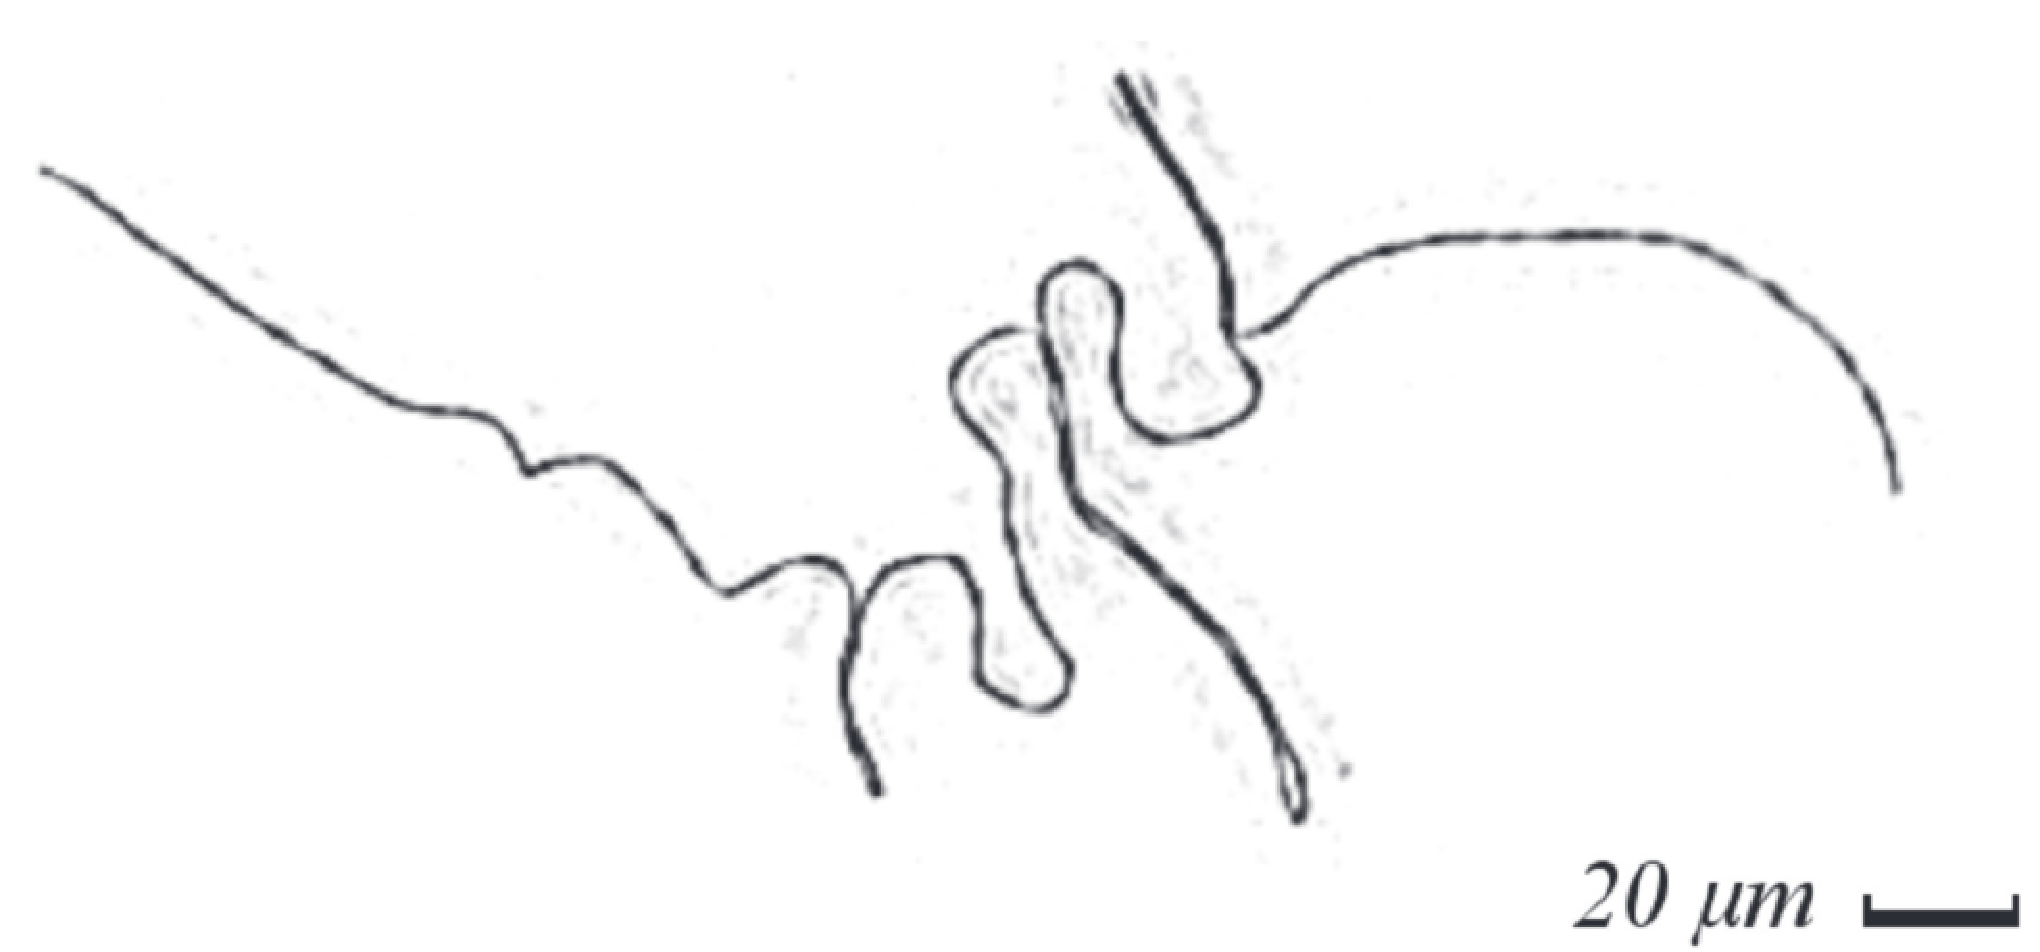
\includegraphics[width=0.5\textwidth]{../img/folding.pdf}
\caption{バクテリア細胞のひも状構造のスナップショット $^{2)}$}
\end{figure}

\end{frame}%}}}

\begin{frame}{研究背景} %{{{

\begin{figure}[htbp]
\centering
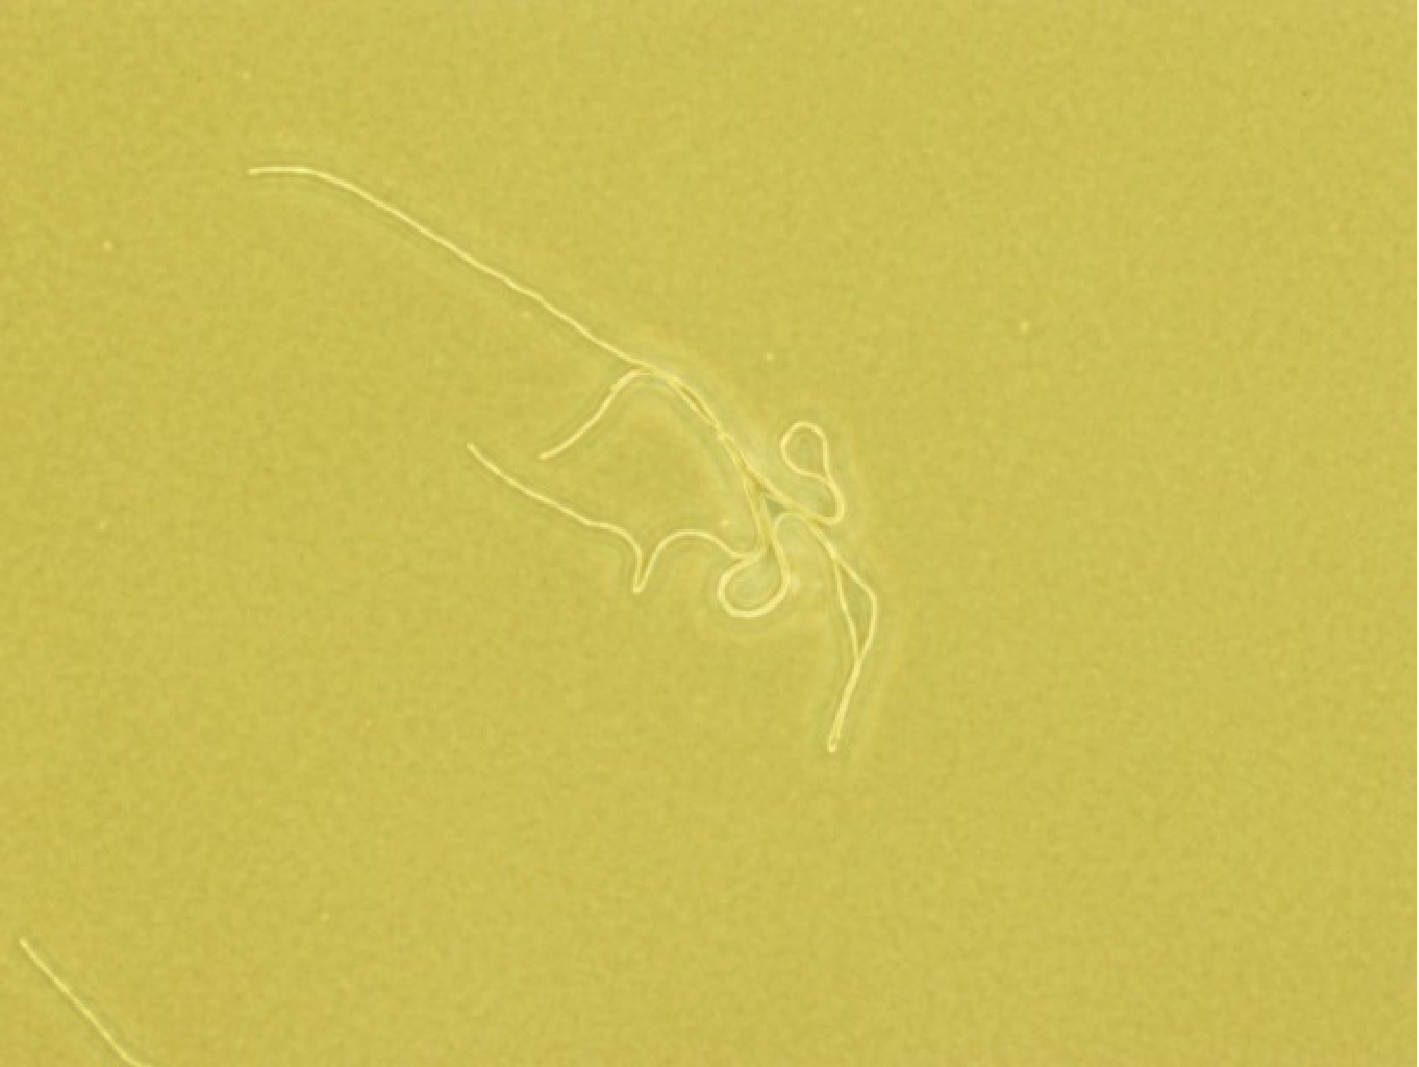
\includegraphics[width=0.7\textwidth]{../img/fold_real.pdf}
\caption{バクテリア細胞の時間発展(脇田研により撮影。x20, 900倍速)}
\end{figure}

\end{frame}%}}}
%}}}
\section{研究目的} %{{{
\begin{frame}{研究目的} %{{{

\begin{itemize}
\itemsep1pt\parskip0pt\parsep0pt
\item
  2次元平面内でのひも状オブジェクトの挙動を記述するモデルを作成

  \begin{itemize}
  \itemsep1pt\parskip0pt\parsep0pt
  \item
    寒天培地上での細胞の成長の記述
  \item
    全長の指数関数的成長,k-folding領域の長さに関する微分方程式の解の挙動を再現
  \end{itemize}
\item
  平面上の1次元ひも状オブジェクトと見なせる他の現象の記述

  \begin{itemize}
  \itemsep1pt\parskip0pt\parsep0pt
  \item
    Viscous fingering
  \item
    Rayleigh--Taylor不安定性
\end{itemize}
\end{itemize}

\end{frame}%}}}
%}}}
\section{モデル}%{{{

\begin{frame}{モデル}%{{{

いくつかのモデルを作成

\begin{itemize}
  \itemsep1pt\parskip0pt\parsep0pt
  \item
    ひも状細胞を弾性体としてとらえるモデル

    \begin{itemize}
      \itemsep1pt\parskip0pt\parsep0pt
      \item
        自然長増大による成長
      \item
        自然長,バネ定数を一定に保つモデル
    \end{itemize}
  \item
    三角格子上で動くひも状オブジェクトのモデル
\end{itemize}

\end{frame}%}}}

\subsection{ひも状細胞を弾性体としてとらえるモデル}%{{{
      \begin{frame}{ひも状細胞を弾性体としてとらえるモデル}%{{{
        \begin{itemize}
          \itemsep1pt\parskip0pt\parsep0pt
          \item
            $N$個の質点がそれぞればねで1次元的に繋がれている
          \item
            ばねの伸びによるフック則に従う力$F^{s}$
          \item
            曲げ弾性による力$F^{b}$
        \end{itemize}

        \begin{figure}[H]
          \begin{center}
            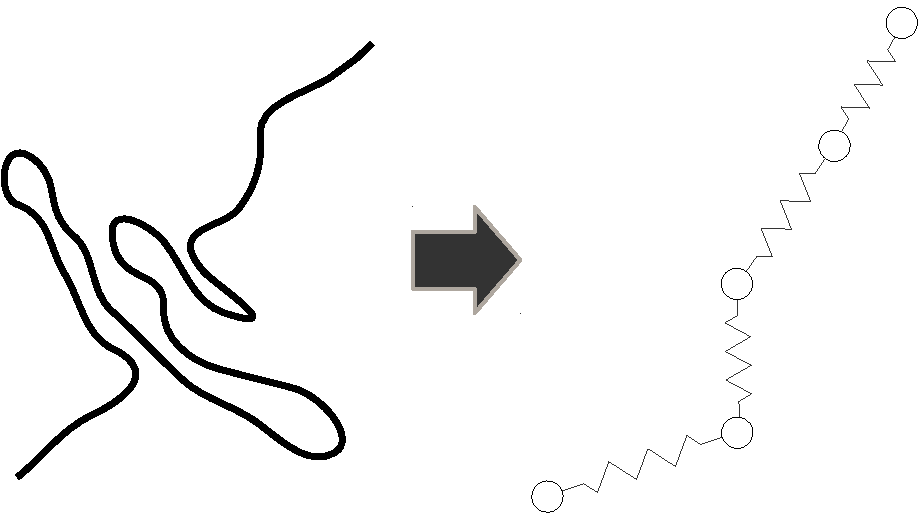
\includegraphics[width=0.5\textwidth]{../img/model.pdf}
            \caption{ひも状細胞の質点とばねによるモデル化}
            \label{fig:model}
          \end{center}
        \end{figure}

        運動方程式を立てて,オイラー法などで数値的に計算する

      \end{frame}%}}}

      \begin{frame}{各質点に対する運動方程式}%{{{
              $i$番目($i \in [0, N-1]$)の質点($m=1$)に関する運動方程式
        \begin{align*}
          \ddot{\vector{r}}_{i} &= F_{i}^{s} + F_{i}^{b} - \gamma \dot{\vector{r}}_{i}
          \tag{1}\label{e1} \\
          \\
          F_{i}^{s} &= - K_{i-1}(d_{i-1} - n_{i-1}) + K_{i}(d_{i} - n_{i}) 
          \tag{1.a}\label{e1a} \\
          F_{i}^{b} &= E_i\left(\frac{\vector{r}_{i-1} + \vector{r}_{i+1}}{2} - \vector{r}_{i}\right) \\
          &\quad  - \frac{1}{2} E_{i-1}\left(\frac{\vector{r}_{i-2} + \vector{r}_{i+2}}{2} - \vector{r}_{i-1}\right) \\
          &\quad - \frac{1}{2}E_{i+1}\left(\frac{\vector{r}_{i} + \vector{r}_{i+2}}{2} - \vector{r}_{i+1}\right)
          \tag{1.b}\label{e1b}
        \end{align*}
      \end{frame}%}}}

      \begin{frame}{各質点に対する運動方程式}%{{{
          \begin{figure}[H]
            \begin{center}
              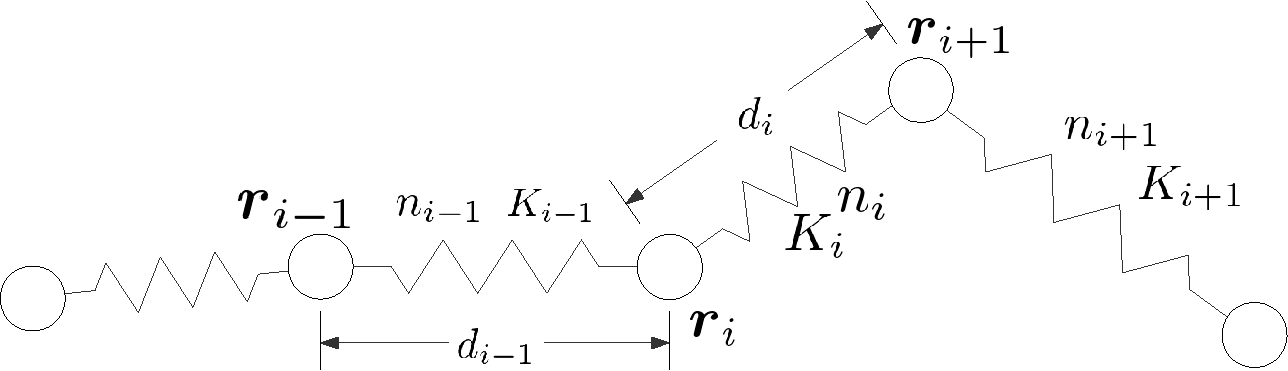
\includegraphics[width=0.7\textwidth]{../img/coordinates.pdf}
              \vspace{0.5cm}
              \caption{質点とばねに関する物理量}
              \label{fig:coodinates}
            \end{center}
          \end{figure}
          \begin{align*}
            \vector{r}_{i} &: i\text{番目の質点の位置ベクトル} \\
            K_{i} &: i\text{番目と}i+1\text{番目の質点間のバネのバネ定数} \\
            n_{i} &: i\text{番目と}i+1\text{番目の質点間のバネの自然長} \\
            d_{i} &: i\text{番目と}i+1\text{番目の質点間の距離} \\
            E_{i} &: i-1,i,i+1\text{番目の3つの質点により決まる曲げ弾性係数}
          \end{align*}
      \end{frame}%}}}

      \begin{frame}{各質点に対する運動方程式}%{{{
              \begin{itemize}
                \itemsep1pt\parskip0pt\parsep0pt
                \item
                  ひもの先端と終端がつながっている場合 ($=$\textbf{閉}):

                  \begin{itemize}
                    \itemsep1pt\parskip0pt\parsep0pt
                    \item
                      $K_{-1}$や$n_{-1}$,$d_{-1}$,$E_{0}$,$E_{N}$は質点$0$と質点$N-1$の間で定義
                  \end{itemize}
                \item
                  ひもの先端と終端が繋がれていない場合 ($=$\textbf{開}):

                  \begin{itemize}
                    \itemsep1pt\parskip0pt\parsep0pt
                    \item
                      $K_{-1} = E_{0} = E_{N-1} = 0$と再定義
                  \end{itemize}
              \end{itemize}
      \end{frame}%}}}

      \begin{frame}{行列式への変換}%{{{
        \begin{itemize}
          \itemsep1pt\parskip0pt\parsep0pt
          \item
            $\vector{x}$: $x$座標に関する配列
          \item
            $\vector{y}$: $y$座標に関する配列
          \item
            $\dot{\vector{x}}$: $x$方向の速度の配列
          \item
            $\dot{\vector{y}}$: $y$方向の速度の配列
        \end{itemize}

        $F_{i}^{s}$を$x$成分と$y$成分で分けて考えると,
        \begin{eqnarray*}
          F_{x_{i}}^{s} = Z_{i} \cdot \vector{x}, \quad F_{y_{i}}^{s} = Z_{i} \cdot \vector{y}
        \end{eqnarray*}
        このとき
        \begin{eqnarray*}
          Z_{i} = \left(
            \begin{array}{ccccccc}
              \cdots &  0 & -z_{i-1} & z_{i-1} + z_{i} & - z_{i} & 0 & \cdots
            \end{array}
          \right)\ \ 
          \text{ただし }z_{i} \equiv K_{i}\left( \frac{n_{i}}{d_{i}} - 1\right)
        \end{eqnarray*}

        よって
        \begin{eqnarray*}
          F_{x}^{s} = Z \cdot \vector{x}, \quad F_{y}^{s} = Z \cdot \vector{y}.
        \end{eqnarray*}
      \end{frame}%}}}

      \begin{frame}{行列式への変換}%{{{

        \begin{eqnarray*}
          Z = \left(
            \begin{array}{ccccccc}
              z_{-1} + z_{0} & -z_{0}        & 0      & \cdots & \cdots   & 0                 & -z_{-1}          \\
              -z_{0}         & z_{0} + z_{1} & -z_{1} & 0      & \cdots   & \cdots            & 0                \\
              0              & \ddots        & \ddots & \ddots & 0        & \cdots            & 0                \\
              \vdots         & \vdots        & \vdots & \vdots & \vdots   & \vdots            & \vdots           \\
              0              & \cdots        & \cdots & 0      & -z_{N-3} & z_{N-3} + z_{N-2} & -z_{N-2}         \\
              -z_{-1}        & 0             & \cdots & \cdots & 0        & -z_{N-2}          & z_{N-2} + z_{N-1}
            \end{array}
          \right)_{.}
        \end{eqnarray*}
      \end{frame} %}}}

      \begin{frame}{行列式への変換}%{{{
        \begin{eqnarray*}
          z = \left(
            \begin{array}{ccccc}
              z_{-1} & 0      & \cdots & \cdots  & 0       \\
              0      & z_{0}  & 0      & \cdots  & 0       \\
              0      & \cdots & \ddots & \cdots  & 0       \\
              0      & \cdots & 0      & z_{N-3} & 0       \\
              0      & \cdots & \cdots & 0       & z_{N-2}
            \end{array}
          \right)_{,} \quad
          z^{u} = \left(
            \begin{array}{ccccc}
              0      & z_{0}  & 0      & \cdots  & 0       \\
              0      & \cdots & \ddots & \cdots  & 0       \\
              0      & \cdots & 0      & z_{N-3} & 0       \\
              0      & \cdots & \cdots & 0       & z_{N-2} \\
              z_{-1} & 0      & \cdots & \cdots  & 0
            \end{array}
          \right)
        \end{eqnarray*}
        \begin{eqnarray*}
          z^{l} = \left(
            \begin{array}{ccccc}
              0      & \cdots & \cdots  & 0       & z_{-1} \\
              z_{0}  & 0      & \cdots  & 0       & 0      \\
              \cdots & \ddots & \cdots  & 0       & 0      \\
              \cdots & 0      & z_{N-3} & 0       & 0      \\
              \cdots & \cdots & 0       & z_{N-2} & 0
            \end{array}
          \right)_{,} \quad
          z^{ul} = \left(
            \begin{array}{ccccc}
              z_{0} & 0      & \cdots & \cdots  & 0       \\
              0      & z_{1}  & 0      & \cdots  & 0       \\
              0      & \cdots & \ddots & \cdots  & 0       \\
              0      & \cdots & 0      & z_{N-2} & 0       \\
              0      & \cdots & \cdots & 0       & z_{N-1}
            \end{array}
          \right)
        \end{eqnarray*}
        のように表すことにすると,
        $$Z = z + z^{ul} - z^{u} - z^{l}$$
      \end{frame}%}}}

      \begin{frame}{行列式への変換}%{{{
        同じように,曲げ弾性による力$F_{i}^{b}$を$x$成分と$y$成分で分けて考えると,
        \begin{eqnarray*}
          F_{x_{i}}^{s} = B_{i} \cdot \vector{x}, \quad F_{y_{i}}^{s} = B_{i} \cdot \vector{y}
        \end{eqnarray*}
        \begin{eqnarray*}
          B_{i}^{T} = \left(
            \begin{array}{c}
              \vdots \\
              0 \\
              -\frac{1}{4}E_{i-1} \\
              \frac{1}{2}E_{i} + \frac{1}{2}E_{i-1} \\
              -E_{i} - \frac{1}{4}E_{i-1}-\frac{1}{4}E_{i+1} \\
              \frac{1}{2}E_{i} + \frac{1}{2}E_{i+1}\\
              -\frac{1}{4}E_{i+1} \\
              0 \\
              \vdots
            \end{array}
            \right)
        \end{eqnarray*}

      \end{frame}%}}}

      \begin{frame}{行列式への変換}%{{{
        これを$z$と同様に行列$e$
        \begin{eqnarray*}
          e = \left(
            \begin{array}{ccccc}
              E_{-1} & 0      & \cdots & \cdots  & 0       \\
              0      & E_{0}  & 0      & \cdots  & 0       \\
              0      & \cdots & \ddots & \cdots  & 0       \\
              0      & \cdots & 0      & E_{N-3} & 0       \\
              0      & \cdots & \cdots & 0       & E_{N-2}
            \end{array}
          \right)
        \end{eqnarray*}

と,その上下左右へ要素を平行移動した行列$e^{l}$,$e^{d}$,$e^{r}$,$e^{u}$,$e^{ld}$,$e^{rd}$,$e^{lu}$,$e^{ru}$を考えると,

$$B = -\frac{1}{4}\left(e^{ld} + e^{rd} + e^{lu} + e^{ru}\right) + \frac{1}{2}\left( e^{l} + e^{d} + e^{r} + e^{u} \right) - e$$

となる.

      \end{frame} %}}}
%}}}

\subsubsection{自然長増大による成長}%{{{
      \begin{frame}{自然長増大}%{{{
        \begin{itemize}
          \itemsep1pt\parskip0pt\parsep0pt
          \item
            ひも状オブジェクトの成長を記述するために,バネの自然長が増大するようにする
          \item
            自然長がある閾値を超えた時,その線分要素を内分する新たな点を追加($\Rightarrow$増殖)
          \item
            $n_{k}$: 時刻$t_{k},\ (k = 0, 1, \dots ,n)$における自然長
            \begin{eqnarray*}
              n_{k + 1} = n_{k} + \alpha \Delta t_{k}
            \end{eqnarray*}
            $\alpha$: 単位時間あたりの自然長の成長率
          \item 線分の単位長さあたりのエネルギーが保存されるように\\
          各時刻におけるバネ定数$K_{k}$を
$$K_{k+1} = K_{k} n_{k} / n_{k+1}$$
          のように補正
        \end{itemize}
      \end{frame}%}}}

      \begin{frame}{分裂時の操作(位置,速度)}%{{{

        自然長がある一定の閾値($n_{c}$)を超え,点を追加する際に更新される物理量

        \begin{itemize}
          \itemsep1pt\parskip0pt\parsep0pt
          \item
            質点の速度
          \item
            自然長
          \item
            バネ定数
        \end{itemize}

        二つの質点の中点の座標に新たな質点を追加する:
        \[\vector{r}_{j} = \frac{\vector{r}_{i+1} + \vector{r}_{i}}{2}\]

        \begin{itemize}
          \itemsep1pt\parskip0pt\parsep0pt
          \item
            新たに追加する点の速度は両端の2点の速度の平均
          \item
            運動量の保存 追加した点に与えた分だけ2点は運動量を失う
        \end{itemize}
        \begin{eqnarray*}
          \left\{
            \begin{array}{rl}
              \vector{v}_{j}^{k+1} &= \frac{\vector{v}_{i}^{k} + \vector{v}_{i+1}^{k}}{2} \\\\
              \vector{v}_{i}^{k+1} &= \vector{v}_{i}^{k} - \frac{1}{2}\vector{v}_{i+1}^{k} \\\\
              \vector{v}_{i+1}^{k+1} &= \vector{v}_{i+1}^{k} - \frac{1}{2}\vector{v}_{i}^{k}
            \end{array}\right.
          \end{eqnarray*}
        \end{frame}%}}}

      \begin{frame}{分裂時の操作(自然長,バネ定数)}%{{{
        分断された二つのばねの長さの比が次の自然長の比となる\\
        今の場合分割された二つのばねの自然長は,分裂前の自然長の1/2
        \begin{eqnarray*}
          n_{j}^{k+1} = n_{j+1}^{k+1} = \frac{n_{i}^{k}}{2}
        \end{eqnarray*}

        分裂の前後でエネルギー保存\\
        \begin{eqnarray*}
          K_{j}^{k+1} = K_{j+1}^{k+1} = 2 K_{i}^{k}
        \end{eqnarray*}
      \end{frame}%}}}
%}}}

\subsubsection{結果}%{{{
      \begin{frame}{実演}%{{{

      \end{frame}%}}}

      \begin{frame}{シミュレーション結果}%{{{
        \begin{figure}[htbp]
          \centering
          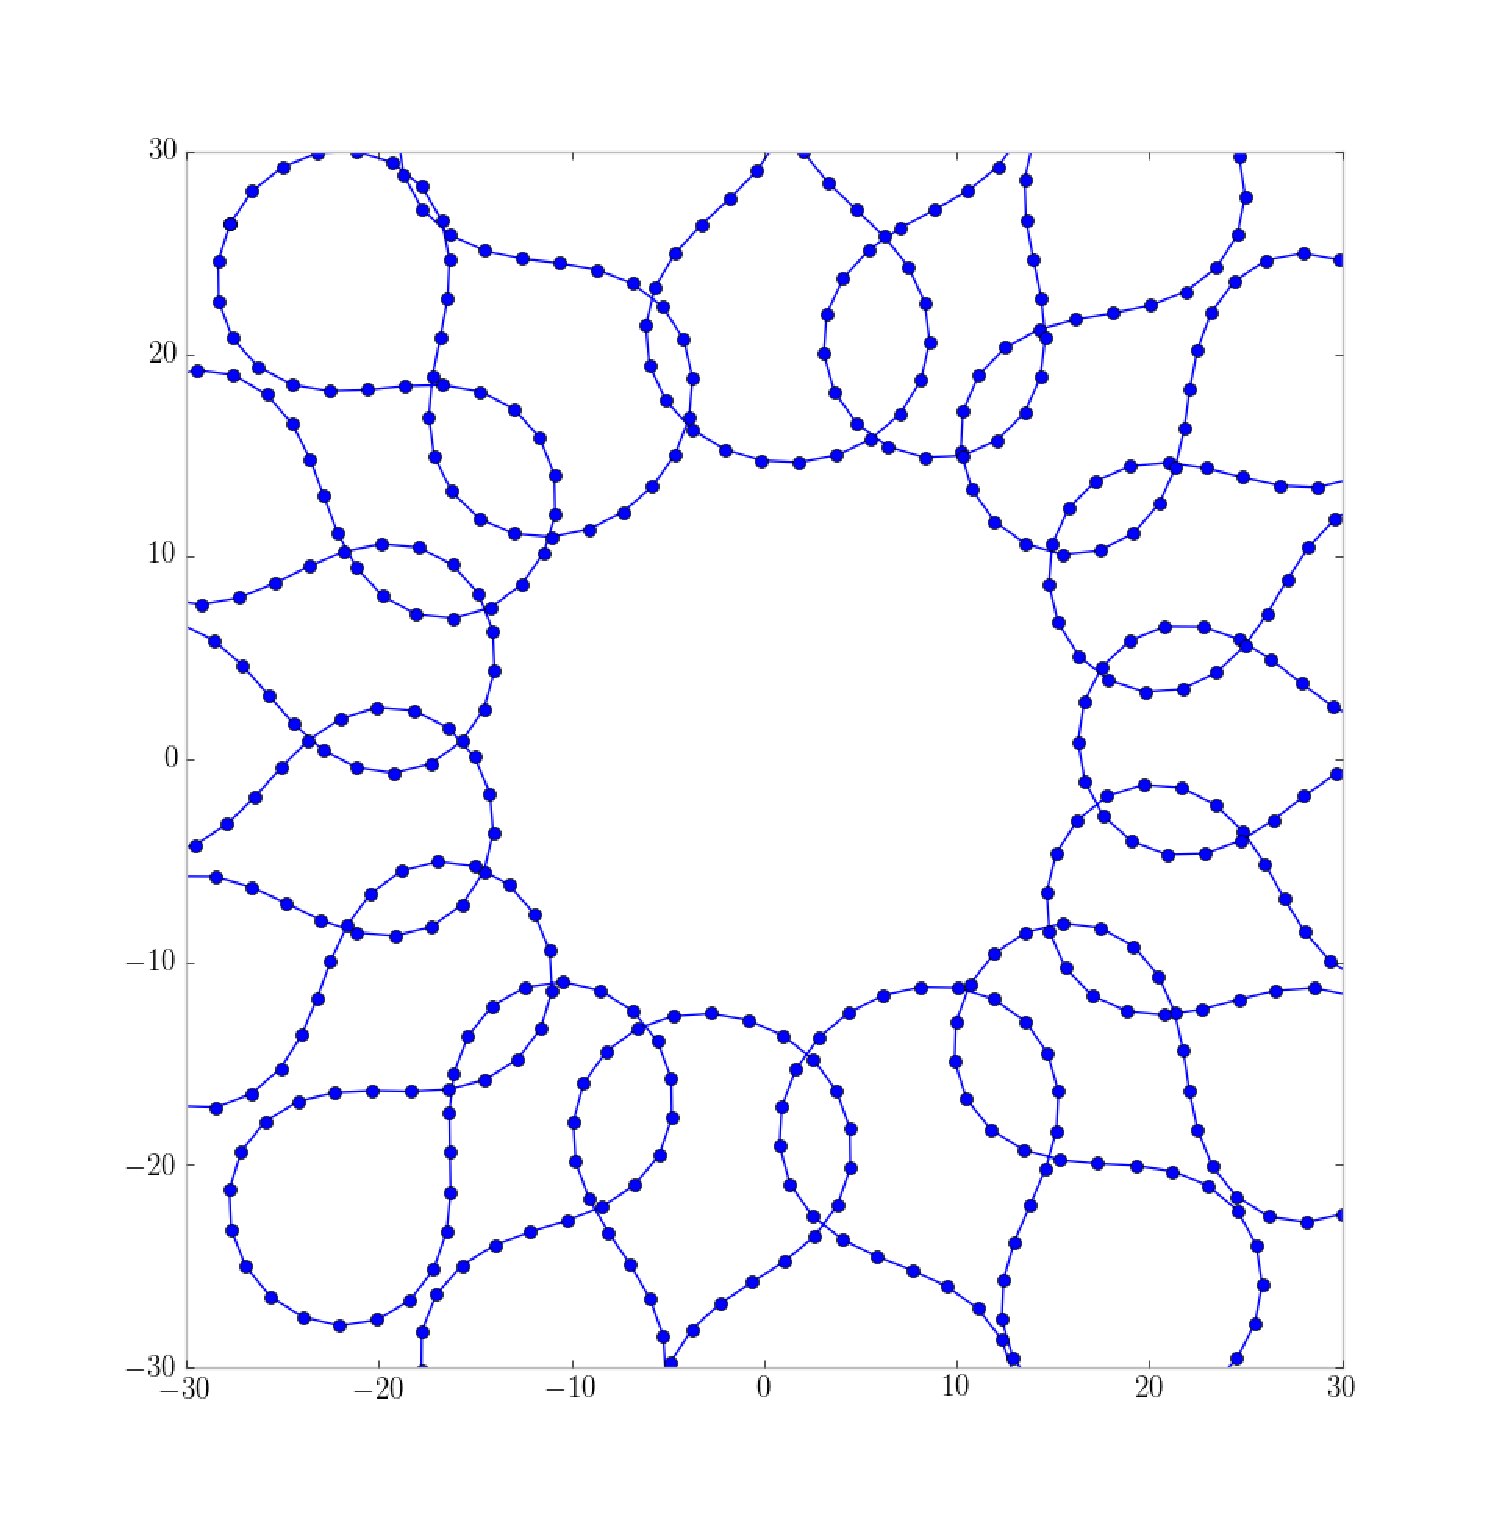
\includegraphics[width=0.5\textwidth]{../img/figure_1.pdf}
          \caption{閉条件でシミュレーションを行った場合}
        \end{figure}
      \end{frame}%}}}

      \begin{frame}{シミュレーション結果のまとめ}%{{{
        \begin{itemize}
          \itemsep1pt\parskip0pt\parsep0pt
          \item
            適切なバネ定数,弾性係数を設定する必要がある
          \item
            バネの本数は倍々に増え,全体の長さは指数関数的に増えていると見なせるかもしれない
          \item
            1回折れ曲がってできた2本のひも状構造がくっつきながら成長していく振る舞いは観察されない\\
            $\because$バネの重なりを許しているため
        \end{itemize}
      \end{frame}%}}}

      \begin{frame}{自己排他性を追加した場合}%{{{
        各バネの交差が起こらないようにルールを変更
        \begin{itemize}
          \itemsep1pt\parskip0pt\parsep0pt
          \item
            質点位置の更新のタイミングで交差判定を行う
          \item
            交差している箇所について,その交差を解消するように新しく移動後の点を取り直す
          \item
            他の箇所に対しても再度交差判定を行う
          \item
            最終的に交差した箇所がなくなるまで過程を続ける
          \item
            この間に時間ステップは進めず,最終的な配置が決定してから時間ステップを1進める
        \end{itemize}
      \end{frame}%}}}

      \begin{frame}{自己排他性を追加した場合}%{{{
        うまくいっていない。

        \begin{itemize}
          \itemsep1pt\parskip0pt\parsep0pt
          \item
            一般的には剛体球ポテンシャルなどを仮定

            \begin{itemize}
              \itemsep1pt\parskip0pt\parsep0pt
              \item
                自然長が増大+長さ一定の保証なし $\rightarrow$ 線分の交差判定
              \item
                (と思っていたが,自然に実装できる?)
            \end{itemize}
          \item
            交差解消が無限ループ
        \end{itemize}

      \end{frame}%}}}
%}}}

\subsubsection{自然長,バネ定数を一定に保つモデル}%{{{
      \begin{frame}{自然長,バネ定数を一定に保つモデル}%{{{
        先ほどのモデルの問題点を解決するため
        \begin{itemize}
          \itemsep1pt\parskip0pt\parsep0pt
          \item
            自然長,バネ定数を一定に保つ
          \item
            ある時間間隔ごとにランダムに点を1つずつ追加し,成長を再現
        \end{itemize}
      \end{frame}%}}}
%}}}

\subsubsection{シミュレーション結果}%{{{
      \begin{frame}{シミュレーション結果}%{{{
        (実演)

        うまくいっていない。
        \begin{itemize}
          \itemsep1pt\parskip0pt\parsep0pt
          \item
            点を追加した際にすぐ発散してしまう
          \item
            適切なパラメータと,斥力ポテンシャルの設定が必要
        \end{itemize}
      \end{frame}%}}}
%}}}

\subsection{三角格子上で動くひも状オブジェクトのモデル}%{{{

      \begin{frame}{三角格子状で動くひも状オブジェクトのモデル}%{{{
        \begin{itemize}
          \itemsep1pt\parskip0pt\parsep0pt
          \item
            質点の位置を2次元ユークリッド空間上の点ではなく,\\
            格子間距離が一定となるような2次元格子上の点とする

            \begin{itemize}
              \itemsep1pt\parskip0pt\parsep0pt
              \item
                隣接する質点とは必ず等しい距離を保つことができる
              \item
                格子点を占めることのできる点の数を1つにすることで\\
                自己排他性を担保
            \end{itemize}
          \item
            三角格子を考える(正方格子: 4回対称性, 三角格子: 6回対称性)
        \end{itemize}
      \end{frame}%}}}

%}}}

\subsubsection{三角格子の構成方法}%{{{

  \begin{frame}{三角格子の構成方法}%{{{
    三角格子をプログラム上で扱うのに適した形とするため
    \begin{itemize}
      \itemsep1pt\parskip0pt\parsep0pt
      \item
        内部では行列
      \item
        隣接関係を再定義
      \item
        描画には図\ref{fig:trilattice}のように潰した形を考える
    \end{itemize}

    \begin{figure}[H]
      \begin{center}
        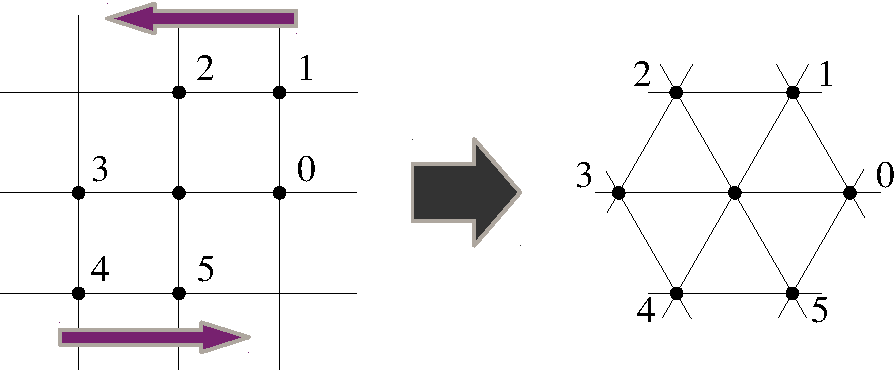
\includegraphics[width=0.7\textwidth]{../img/triangular_lattice.pdf}
        \caption{2次元正方格子を三角格子に対応させるための隣接関係の再定義}
        \label{fig:trilattice}
      \end{center}
    \end{figure}
  また,周期境界条件を課す。
  \end{frame}%}}}
  %}}}

\subsubsection{三角格子状で定義されるひも状オブジェクト}%{{{
      \begin{frame}{ひも状オブジェクトの表現}%{{{
          \begin{itemize}
            \itemsep1pt\parskip0pt\parsep0pt
            \item
              始点となる格子点の座標(正方格子における(行,列))を定める
            \item
              始点から次の格子点へのベクトルを,6方向の単位ベクトル(図\ref{fig:unitvec})\\
              $\vector{u}_{\alpha}\ (\alpha \in \{0, 1, \dots , 5\})$のうちの一つで表現
            \item
              オブジェクトの構成要素数だけベクトルの列を繋げれば,全体が表現できる
          \end{itemize}

          \begin{itemize}
            \itemsep1pt\parskip0pt\parsep0pt
            \item
              ひも状オブジェクト$S$は以下:
              \[ S = ((x, y), (\alpha_{1},  \alpha_{2}, \dots , \alpha_{N-1}) ), \ \alpha_{i} \in \{0, 1, \dots , 5\}\]
          \end{itemize}

          \begin{figure}[H]
            \begin{center}
              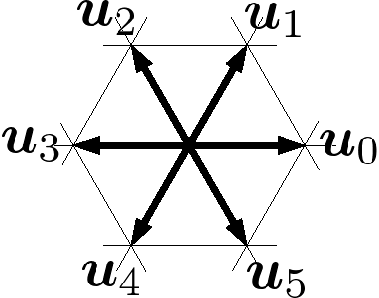
\includegraphics[width=0.3\textwidth]{../img/unitvec.pdf}
              \caption{6つの基本ベクトル}
              \label{fig:unitvec}
            \end{center}
          \end{figure}

        \end{frame}%}}}

%}}}

\subsubsection{ひも状オブジェクトの配置}%{{{

      \begin{frame}{ひも状オブジェクトの格子への配置}%{{{
          重なりなく配置格子点を配置 $\rightarrow$自己回避ランダムウォーク(SAW)の問題

          \begin{enumerate}
          \itemsep1pt\parskip0pt\parsep0pt
          \item
            格子全体から占有されていない点をランダムに一つ選択
          \item
            選択された点の隣接点で占有されていないものへ向かうベクトルを\\
            ランダムに一つ選択
        \end{enumerate}

        以上を繰り返せば良い。

        \textbf{Remark:}

        \begin{itemize}
          \item
            deadlock状態:\\
            構成要素数が多くなり,隣接点がすべて占有されてそれ以上点を増やすことができない状態
          \item
            deadlockとなった時は,一つ前のステップにさかのぼり,将来deadlockする方向のベクトルを除く,占有されていない点に向かうベクトルを選択 (再帰的過程)
        \end{itemize}

        ※
        すべてのパターンを試行してもdeadlockとなる場合,\\
        \ \ \ \ 初期点を選ぶところからやり直す

      \end{frame}%}}}

%}}}

\subsubsection{脱線}%{{{
      \begin{frame}{「成長」を記述するまでの脱線}%{{{
        本来は三角格子上でのひも状オブジェクトの成長を記述するものだが\\
        すこし脱線して三角格子上で遊んでみた

        \begin{itemize}
          \itemsep1pt\parskip0pt\parsep0pt
          \item
            三角格子上のVicsekモデル(本人が論文を書いている)

            \begin{itemize}
              \itemsep1pt\parskip0pt\parsep0pt
              \item
                三角格子上に6方向の単位ベクトルのうち1つを配置していく
              \item
                近隣のベクトルの影響を受けて次の時刻のベクトルの向きを決定
              \item
                温度(ランダムネス)をパラメータとして相転移が見られる
            \end{itemize}
          \item
            ひも状オブジェクトが「頭」からランダムに動く

            \begin{itemize}
              \itemsep1pt\parskip0pt\parsep0pt
              \item
                deadlockしたらそこで終了
              \item
                オブジェクトサイズとdeadlockするまでの時間の関係
              \item
                取りうる配置のうち,$N-1$回deadlockしない配置を選んだ後,$N$回目にdeadlockするパターンを選ぶ試行と統計的に等しい
            \end{itemize}
        \end{itemize}

      \end{frame}%}}}

      \begin{frame}{三角格子上でのVicsekモデル}%{{{

        \begin{figure}[H]
          \begin{center}
            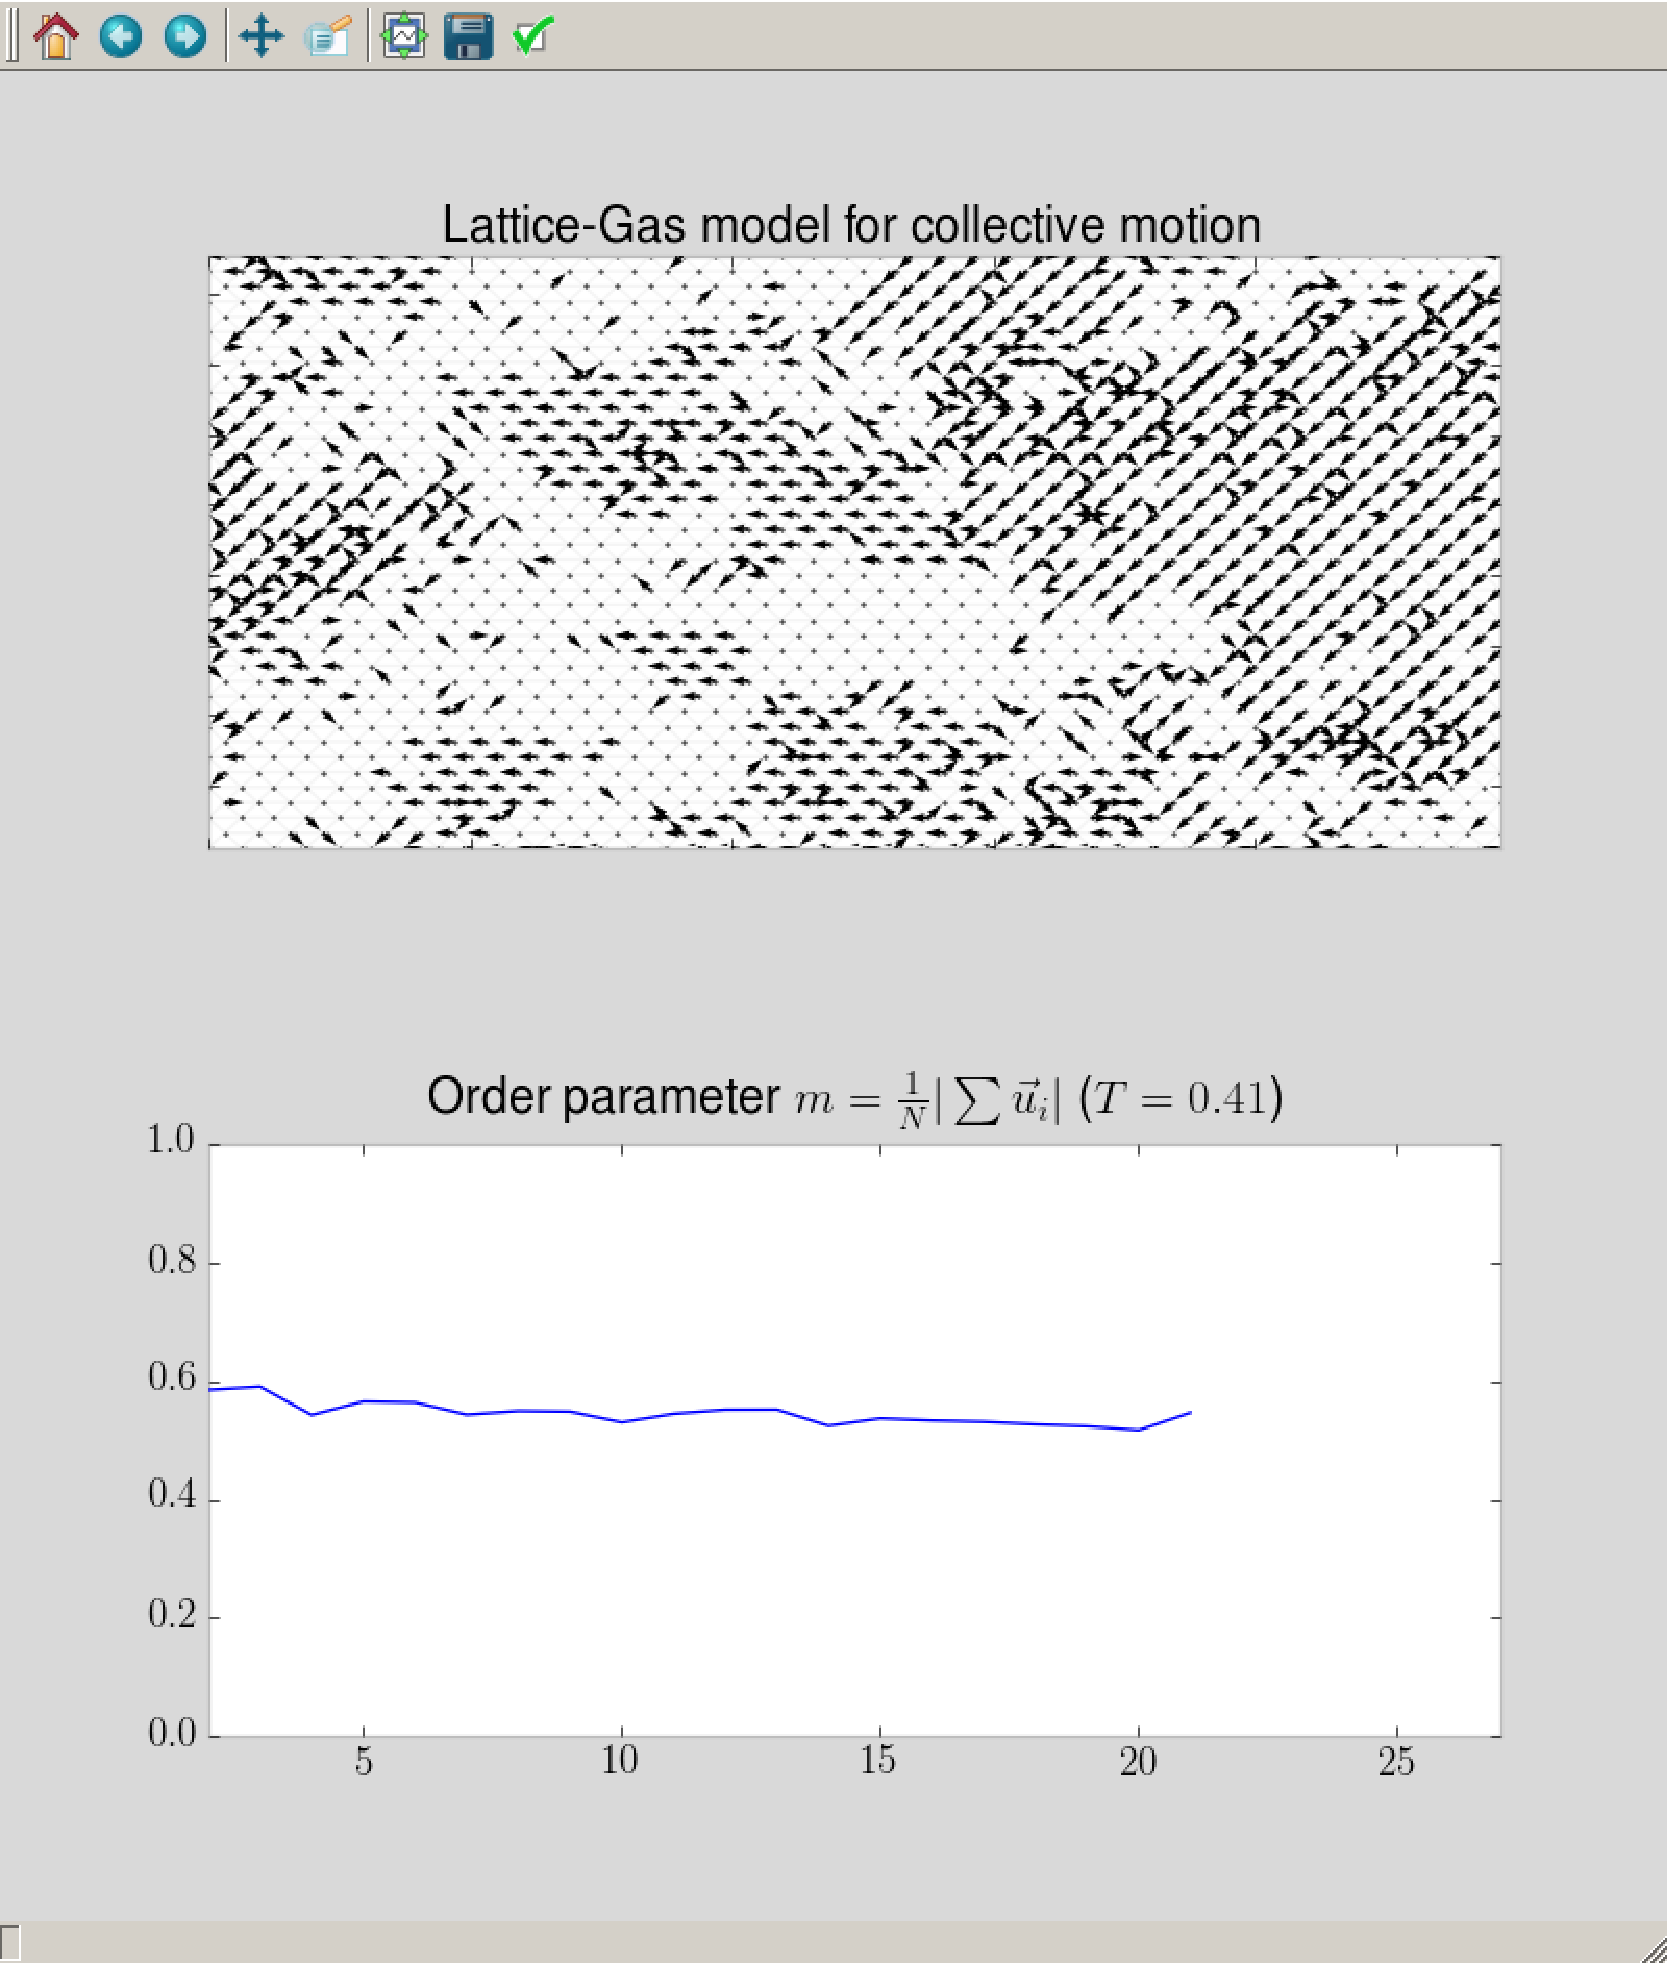
\includegraphics[width=0.45\textwidth]{../img/screen_003.pdf}
            \caption{三角格子上でのVicsekモデルによる集団運動。下段は秩序パラメータを表す。}
          \end{center}
        \end{figure}
      \end{frame}%}}}

      \begin{frame}{三角格子上で動くひも状オブジェクト}%{{{

        \begin{figure}[H]
          \begin{center}
            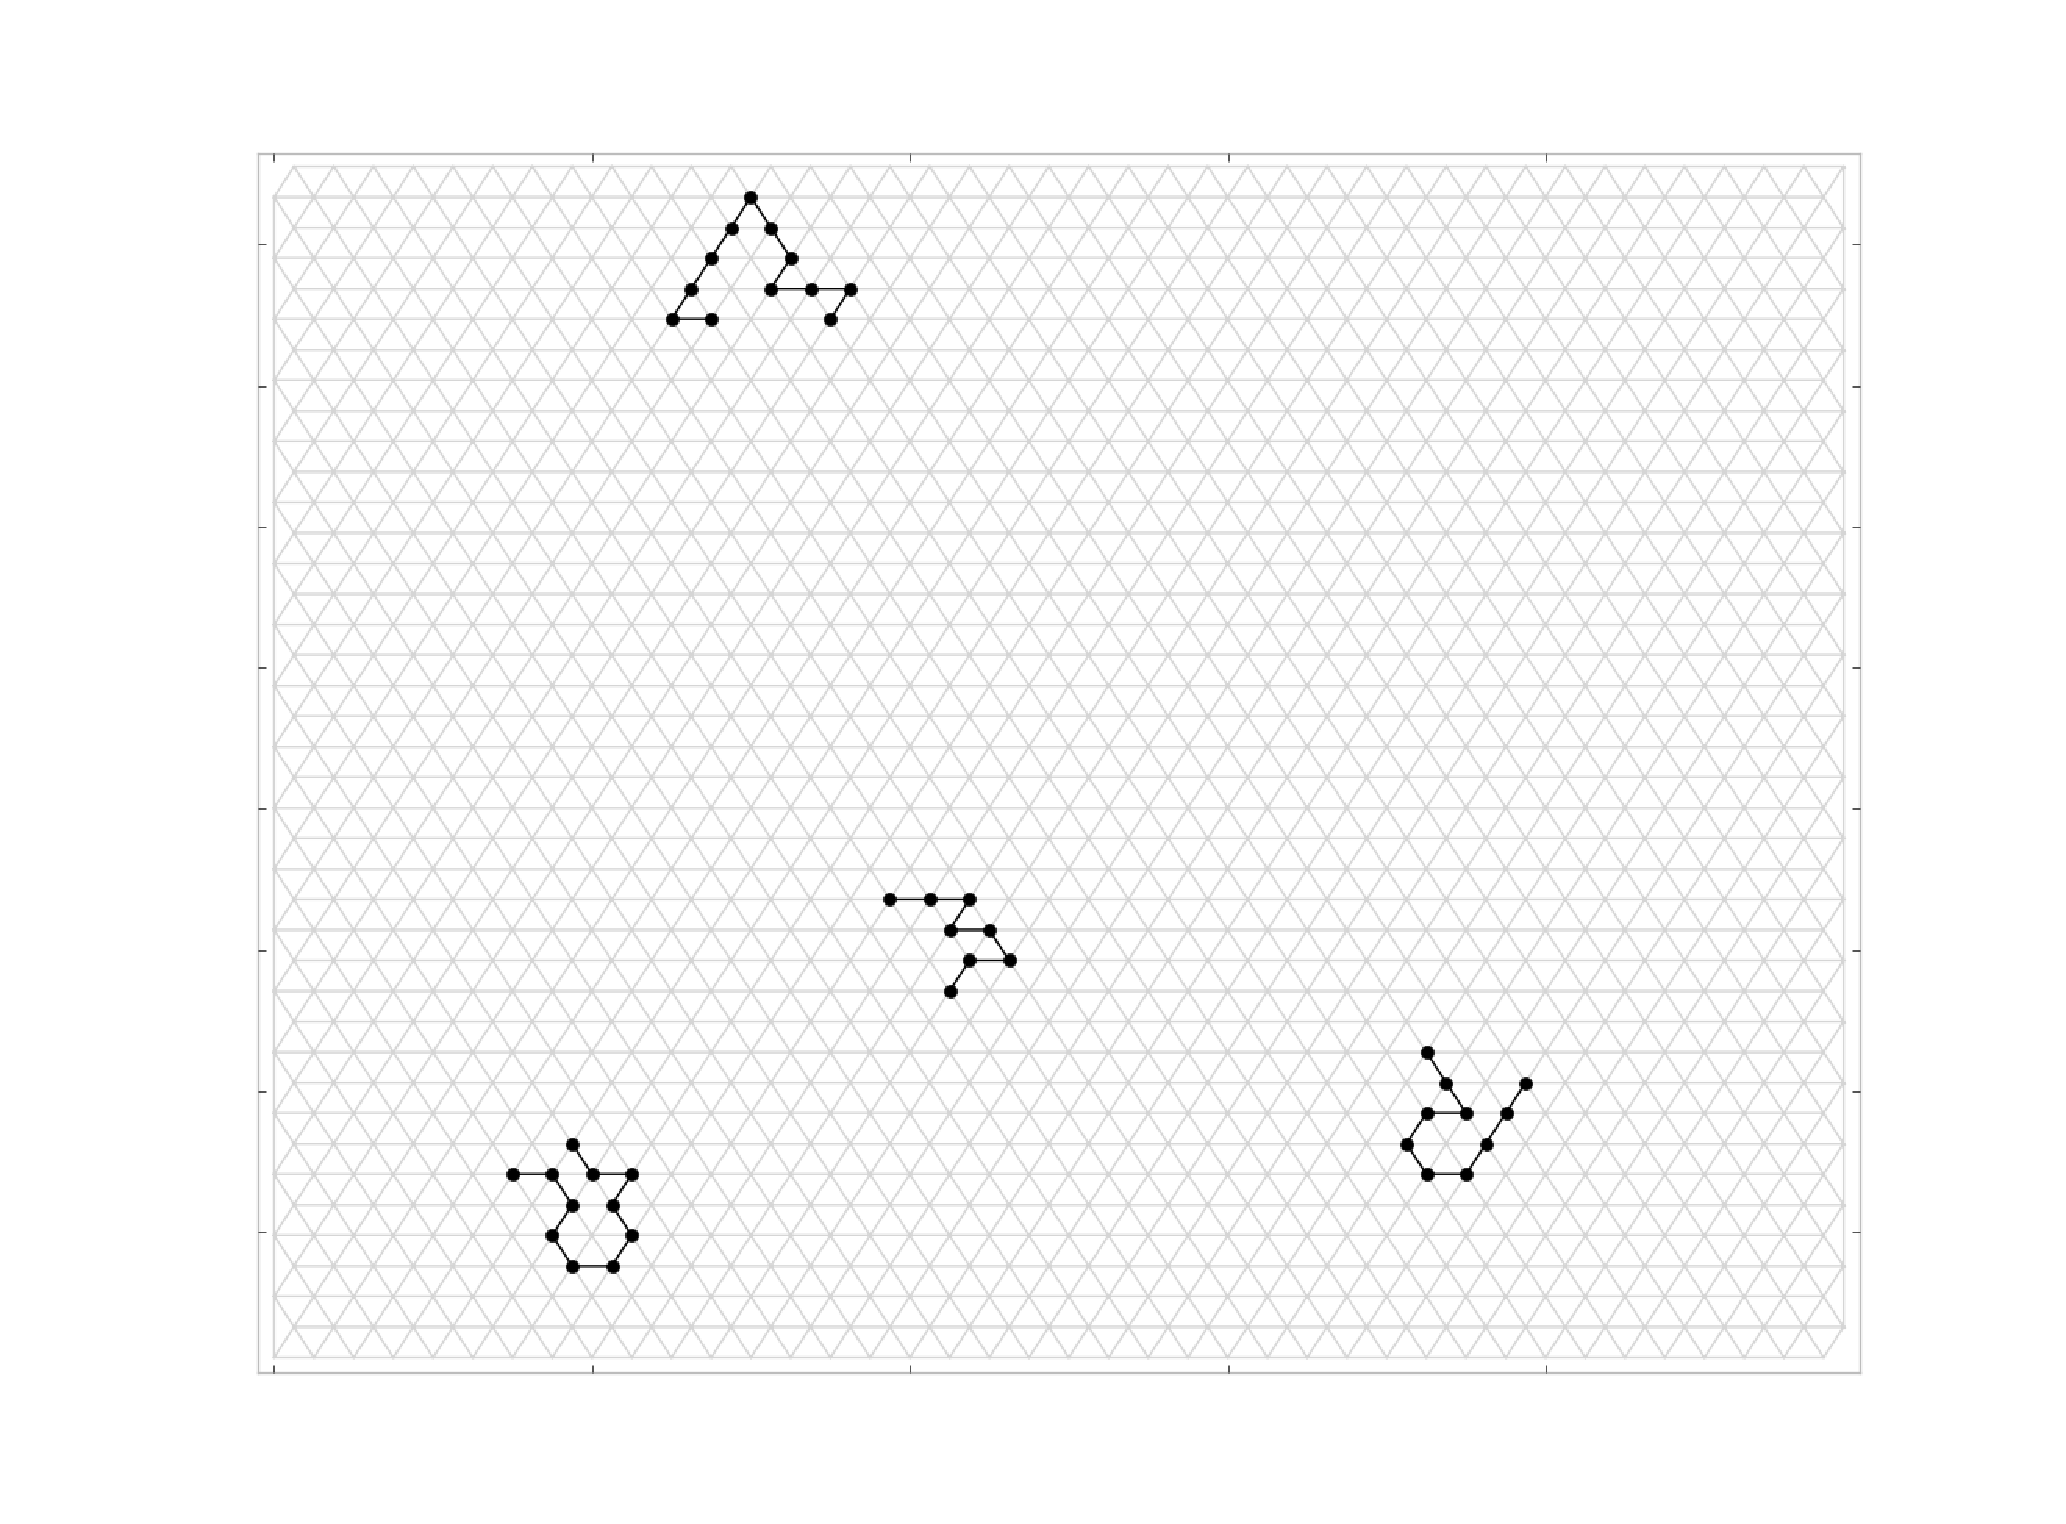
\includegraphics[width=0.7\textwidth]{../img/screen_002.pdf}
            \caption{三角格子上で動くひも状オブジェクト}
          \end{center}
        \end{figure}
      \end{frame}%}}}

%}}}

\subsubsection{三角格子上でのひも状オブジェクトの成長}%{{{
  \begin{frame}{三角格子上でのひも状オブジェクトの成長}%{{{
    WIP ... 
  \end{frame}%}}}
%}}}

%}}}
\section{今後の課題}%{{{
  \begin{frame}%{{{
      \begin{itemize}
        \itemsep1pt\parskip0pt\parsep0pt
        \item
          三角格子上でのひも状オブジェクトの成長
        \item
          自然長増大のモデルで剛体球ポテンシャルを導入

          \begin{itemize}
            \itemsep1pt\parskip0pt\parsep0pt
            \item
              緩和時間より長い間隔で成長すれば,適用可能?
          \end{itemize}
      \end{itemize}
  \end{frame}%}}}
%}}}
\section{参考文献}%{{{
\begin{frame}{参考文献}

\begin{itemize}
\itemsep1pt\parskip0pt\parsep0pt
\item
  \href{http://www.sciencedirect.com/science/article/pii/S0022519397904628}{K.
  Kawasaki, A. Mochizuki, M. Matsushita, T. Umeda, and N. Shigesada.
  Modeling spatio-temporal patterns generated bybacillus subtilis.
  Journal of Theoretical Biology, Vol. 188, No. 2, pp.~177-185, 1997.}
\item
  \href{http://dx.doi.org/10.7566/JPSJ.84.114002}{Ryojiro Honda, Jun
  ichi Wakita, and Makoto Katori. Self-elongation with sequential
  folding of a filament of bacterial cells. Journal of the Physical
  Society of Japan, Vol. 84, No. 11, p.~114002, 2015.}
\item
  \href{http://link.aps.org/doi/10.1103/PhysRevE.52.5297}{Zolt\'an Csah\'ok
  and Tam\'as Vicsek. Lattice-gas model for collective biological motion.
  Phys. Rev.~E, Vol. 52, pp.~5297-5303, November 1995.}
\end{itemize}
\end{frame}

\end{document}%}}}
